\section{Exercise one}

Design an ER Model for a car rental system that manages the customers, the cars and their related elements. 
If a customer wants to rent a car, they should provide their personal ID card (9-digit ID, name,surname, birth date, address, release date, expiration date), driving license (10-digit drive licensenumber, name, surname, birthdate, release date, expiration date and the list of vehicles they are allowed to drive, e.g. truck, car, motorcycle, bus, etc.) and credit card (16 digit number and expiration date). 
Then, the list of cars is shown to the customer. Each car is described by its brand, the price per day, the maximum speed, and the fuel consumption per km. 
Before proposing the car, the system checks whether a car inspection has been performed in the last 3 months. 
Such data includes all the inspections (described by date and the name of the company who took care of it), alongside the list of all the operations the car underwent in each inspection. 
As soon as the customer picks the car they want, the keys are provided to the customer and the system stores the rental invoice (described by rental date, the period for which the car has been rented, and the final price). 
When the car is returned, the customer is charged. 
As soon as the payment is completed, the system marks the rental invoice as closed and the customer is provided with his invoice.

\subsection*{Solution}
We have the following entites (with the corresponding attributes): 
\begin{itemize}
    \item CUSTOMER ID CARD (\underline{ID}, Name, Surname, BirthDate, Address, ReleaseDate, ExpirationDate). 
    \item DRIVING LICENSE (\underline{DriveLicenseNumber}, Name, Surname, BirthDate, ReleaseDate, ExpirationDate, DriveCars, DriveBus). 
    \item CREDIT CARD (\underline{IdentifierNumber}, CVC, ExpirationDate).
    \item CAR (Brand, PricePerDay, MaximumSpeed, FuelConsumption, \underline{LicensePlate}).
    \item CAR INSPECTION (Date, CompanyName, \underline{InspectionID}).
    \item OPERATIONS (\underline{OperationID}, Description). 
    \item RENTAL INVOICE (\underline{RentalInvoiceID}, RentalDate, RentalPeriod, FinalPrice, Status).
    \item CUSTOMER (\underline{E-mail}).
\end{itemize}
To do so we assumed that the Customer is identified through an E-Mail. 
The diagrams of the given problem are: 
\begin{figure}[H]
    \centering
    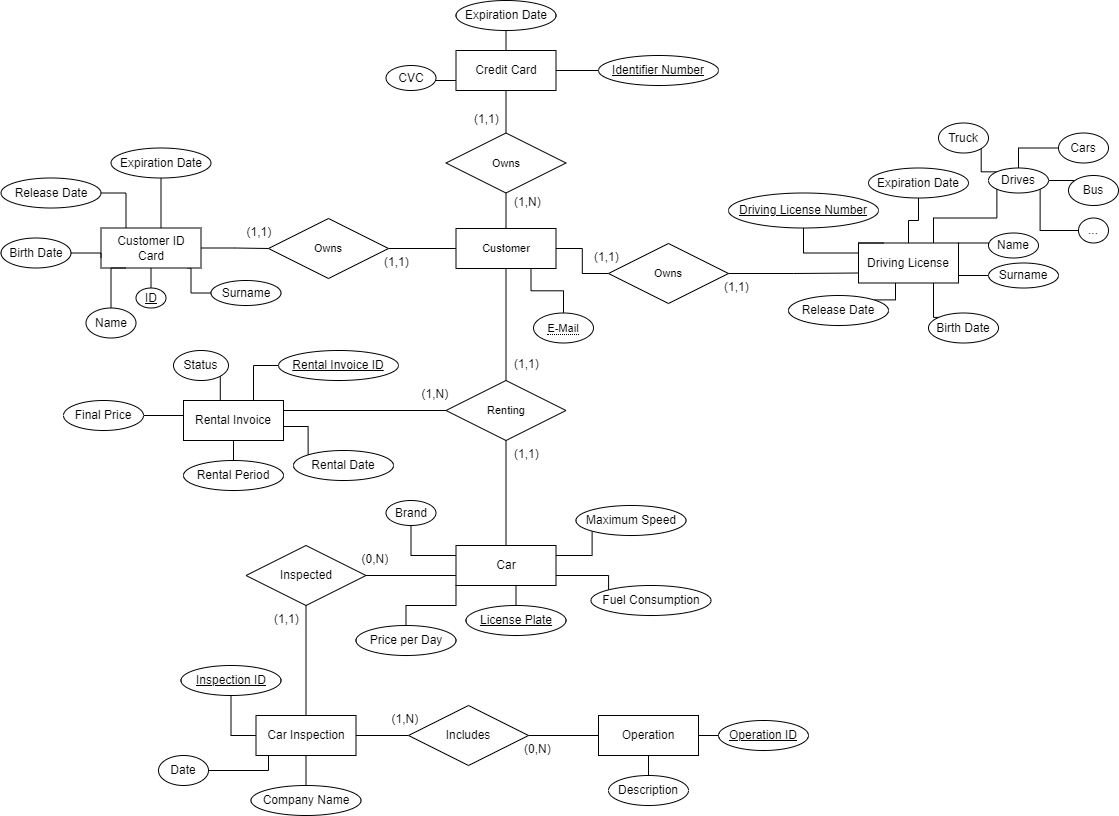
\includegraphics[width=1.00\linewidth]{images/er.png}
\end{figure}